% =============================================================================
%  IV. MATERIALS: DATA AND COHORT        
% =============================================================================
\begin{frame}{IV. Materials: Data and Cohort}
\begin{atucols}[c]
\begin{column}{0.47\textwidth}
  \centering
  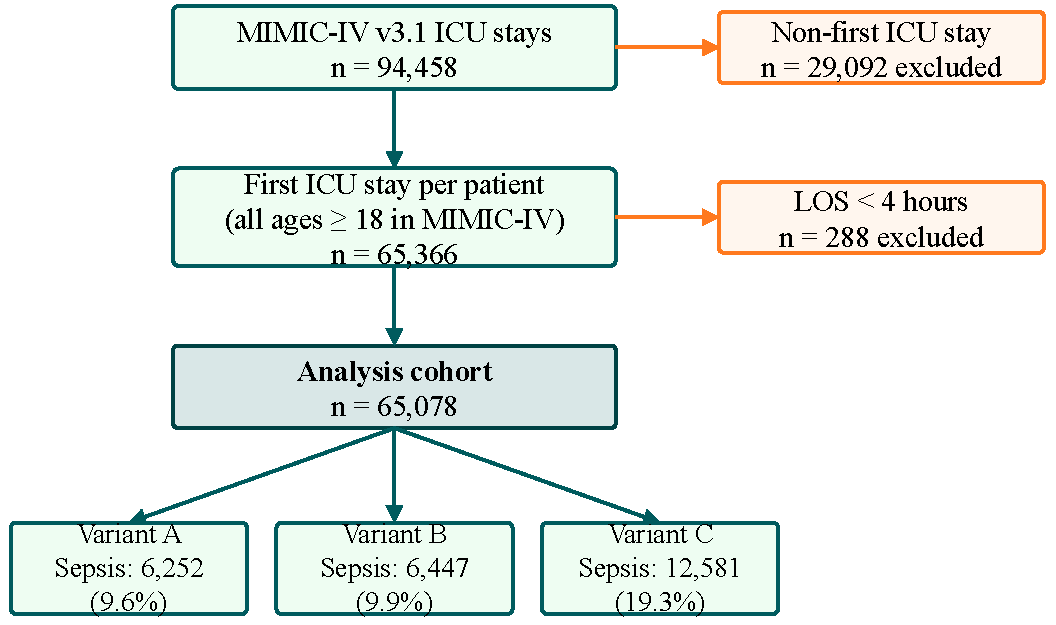
\includegraphics[width=\columnwidth,height=0.74\textheight,
                   keepaspectratio]{images/fig3.1_consort.pdf}
\end{column}
\begin{column}{0.51\textwidth}
\begin{itemize}\itemsep3pt\small
  \item \textbf{Development data:} MIMIC-IV v3.1~\cite{johnson2023mimiciv},
        single centre (BIDMC, Boston).
  \item \textbf{Cohort:} adults, first ICU stay, length of stay $\geq 4$\,h;
        \textbf{n = \pcNStays}.
  \item \textbf{External validation:} eICU-CRD v2.0~\cite{pollard2018eicu};
        \textbf{frozen models, no retraining}.\\
        {\scriptsize\color{MidGrey} over 200 US ICUs, \pcExtNCohortStays{}
        unit stays}
  \item \textbf{Person-hour data:} first 72\,h; discharge and death modelled
        as competing events.
  \item \textbf{22 covariates; \pcNCandidatePredictors{} model terms per
        outcome.}\\
        {\scriptsize\color{MidGrey} 6 vitals, 5 labs, 2 vasopressor flags,
        3 six-hour slopes, 6 test-order indicators}
\end{itemize}
\end{column}
\end{atucols}
\end{frame}


% =============================================================================
%  IV. MATERIALS: THREE SEPSIS-3 LABEL VARIANTS   
% =============================================================================
\begin{frame}{IV. Materials: Three Pre-Registered Sepsis-3 Label Definitions}
\begin{center}\renewcommand{\arraystretch}{1.12}\scriptsize
\begin{tabular}{llcccccr}
\toprule
\textbf{ID} & \textbf{Name} & \textbf{ABX$\to$cx} & \textbf{cx$\to$ABX}
  & \textbf{SOFA$-$} & \textbf{SOFA$+$} & \textbf{Baseline} & \textbf{Septic stays} \\
\midrule
A & Narrow      & 24\,h & 24\,h & 24\,h & 12\,h & Admission     & \pcNOnsetsA{} (\pcPctOnsetsA\%) \\
B & Seymour-Std & 72\,h & 24\,h & 48\,h & 24\,h & Admission     & \pcNOnsetsB{} (\pcPctOnsetsB\%) \\
C & Liberal     & 72\,h & 72\,h & 48\,h & 24\,h & Rolling 24\,h & \pcNOnsetsC{} (\pcPctOnsetsC\%) \\
\bottomrule
\end{tabular}
\end{center}
{\tiny ABX: antibiotic; cx: culture; SOFA$-$/SOFA$+$: permitted hours
before/after suspected infection for a $\geq 2$-point SOFA increase.\par}

\vspace{2pt}
\begin{atucols}[c]
\begin{column}{0.62\textwidth}
\begin{itemize}\itemsep2pt\footnotesize
  \item All definitions require \textbf{suspected infection} (antibiotic
        paired with a culture) \textbf{plus} a $\geq 2$-point SOFA
        increase~\cite{singer2016sepsis3,cohen2024subtle}.
  \item \textbf{B is primary}; A and C are pre-specified alternatives.
  \item Onset is assigned at suspected infection, $t_{\text{susp}}$. SOFA
        determines case membership, not onset time.
\end{itemize}
\vspace{2pt}
\begin{alertblock}{}
  \footnotesize A and B have similar prevalence but low case agreement:
  $\kappa = \pcKappaVsBA$.
\end{alertblock}
\end{column}
\begin{column}{0.36\textwidth}
  \centering
  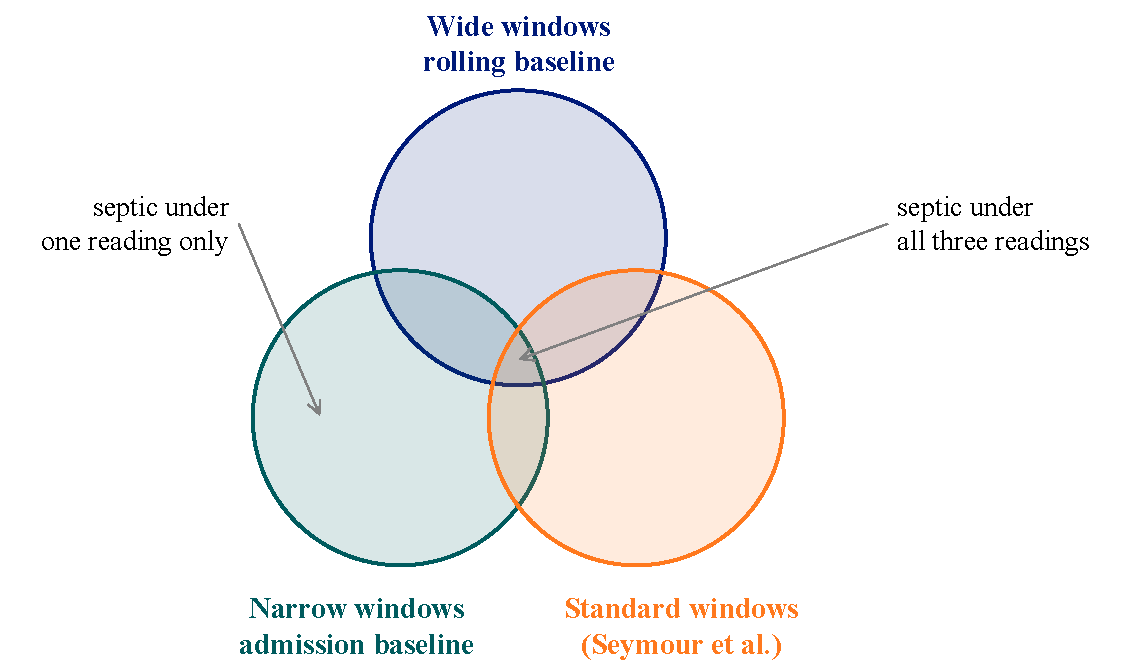
\includegraphics[width=\columnwidth,height=0.42\textheight,
                   keepaspectratio]{images/fig2.2_label_variance_concept.pdf}
\end{column}
\end{atucols}
\end{frame}
